\subsection{AlexNet介绍}
AlexNet 是一个深度卷积神经网络,它的结构如下:\cite{AlexNet}

\begin{figure}[H]
    \centering %表示居中
    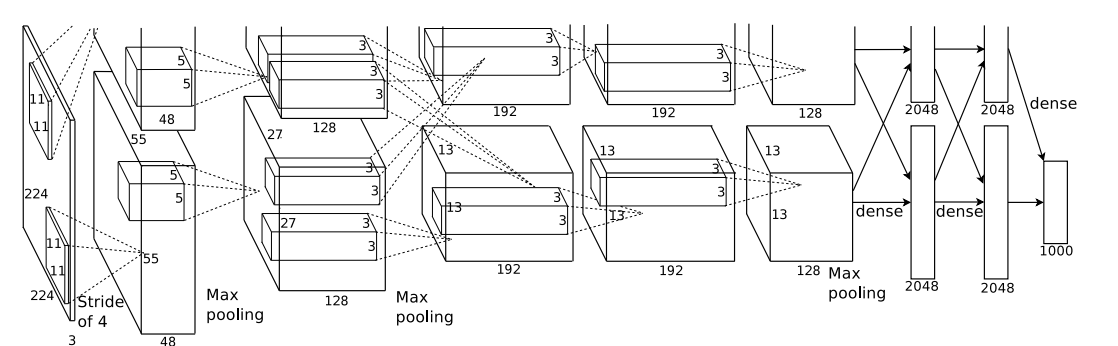
\includegraphics[height=4.5cm]{../../AlexNet/AlexNet_arc.png}
    \caption{AlexNet结构}
\end{figure}

AlexNet 主要特点:\par
1. 更深的网络结构:AlexNet由 5 个卷积层、3 个全连接层和最后的 Softmax 分类层组成。 \par
2. ReLU 激活函数:AlexNet 是第一个大规模使用 ReLU 作为激活函数的网络,这加速了训练过程。 \par
3. Dropout:为了减少过拟合,AlexNet 在全连接层中使用了 Dropout。 \par
4. 局部响应归一化(LRN):在某些卷积层后使用了局部响应归一化。 \par
5. 数据增强:为了进一步减少过拟合,AlexNet 使用了图像平移、翻转和颜色变化等数据增强技术。 \par

\subsection{使用AlexNet对图像进行识别的效果分析}

训练结果如下:
\begin{table}[H]
    \begin{minipage}[b]{0.56\linewidth}
    \centering
    \begin{tabular}{c|c|c}
        \hline
        Epoch & Loss & Test Accuracy \\ \hline \hline
        10 & 1.10 & 46.48 \\ \hline
        20 & 0.75 & 58.00 \\ \hline
        30 & 0.42 & 58.74 \\ \hline
        40 & 0.34 & 57.37 \\ \hline
        50 & 0.13 & 55.33 \\ \hline
       \end{tabular}
        \caption{随训练轮数增加Loss和Test Accuracy的变化}
    \end{minipage}
    \begin{minipage}[b]{0.4\linewidth}
    \centering
    \includegraphics[width=50mm]{../../AlexNet/AlexNet.png}
    \captionof{figure}{AlexNet训练结果}
    \end{minipage}
    \end{table}


% \begin{wrapfigure}{r}{0.3\textwidth}
%     \centering %表示居中
%     \includegraphics[height=4cm]{../AlexNet/AlexNet.png}
%     \caption{AlexNet训练结果}
% \end{wrapfigure}

在训练过程中,我们将数据集按 7:3 的比例划分为训练集和测试集。
采用 AlexNet 进行训练,训练 50 轮后,发现模型对于测试集的预测准确率不断上升,最后趋于稳定,稳定在 55\% 左右;
损失函数值也在不断下降,最终达到了 0.13。考虑到样本集中的数据量只有 2700 左右,数据量偏少,因此训练效果不是很理想。
如果增大样本集规模,模型预测的准确率应该会有进一步提升。 \par
在训练过程中发现,虽然损失函数值在下降,但是预测准确率却并未上升,有时甚至下降,这说明模型可能存在过拟合现象,这也可能是导致模型预测准确率不高的原因之一。
